\chapter{Results and System Demonstration}

\section{Performance Metrics}

\begin{table}[H]
\centering
\resizebox{0.7\textwidth}{!}{
\begin{tabular}{ll}
\toprule
\textbf{Metric} & \textbf{Observed value} \\
\midrule
Route computation (\texttt{/api/route})             & $\sim$ 2 s \\
LLM pipeline (\texttt{/api/disruptions})            & 30 -- 60 s \\
OSM graph load from pickle cache                    & $\sim$ 2 s \\
OSM graph first-time download                       & $\sim$ 30 -- 60 s (once) \\
Data sources integrated                             & 9 \\
Transport modes supported                           & 8 \\
Pre-defined Kolkata localities                      & 15 + metro stations + bus stops \\
Metro lines                                         & 5 \\
Event types extractable                             & 13 \\
HGNN output heads                                   & 3 \\
TomTom free-tier capacity                           & 2{,}500 req/day \\
LLM rate-limit handling                             & Exponential backoff on 429 \\
\bottomrule
\end{tabular}
}
\caption{System performance summary}
\end{table}

% -------------------------------------------------------------------
\section{UI Screenshots}
% -------------------------------------------------------------------

\noindent
\textit{Instructions for compilation: place your \texttt{.png} screenshots
in the same folder as the \texttt{.tex} files and uncomment the relevant
\texttt{\textbackslash includegraphics} line inside each figure environment.}

\bigskip

% -------  Figure 4.1  -------
\begin{figure}[H]
\centering
% Uncomment the line below and replace filename when screenshot is ready:
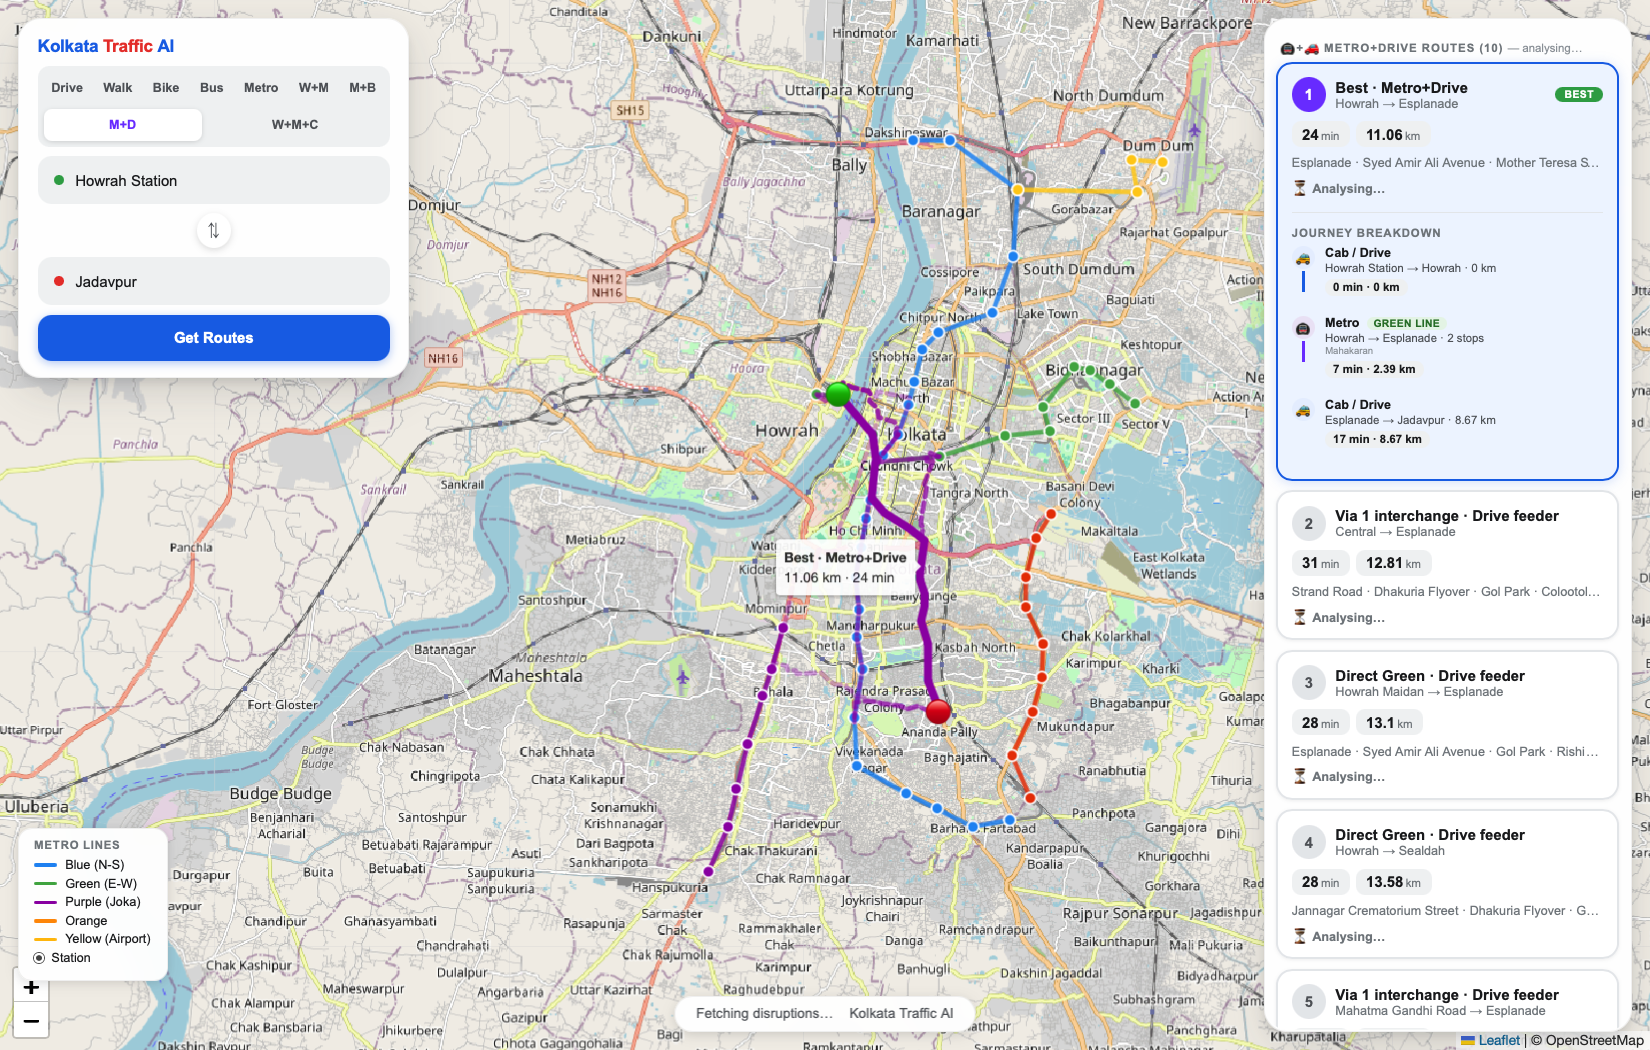
\includegraphics[width=0.8\linewidth]{ui1.png}
\caption{Step~1 --- routes rendered before disruption analysis.}
\label{fig:step1}
\end{figure}

% -------  Figure 4.2  -------
\begin{figure}[H]
\centering
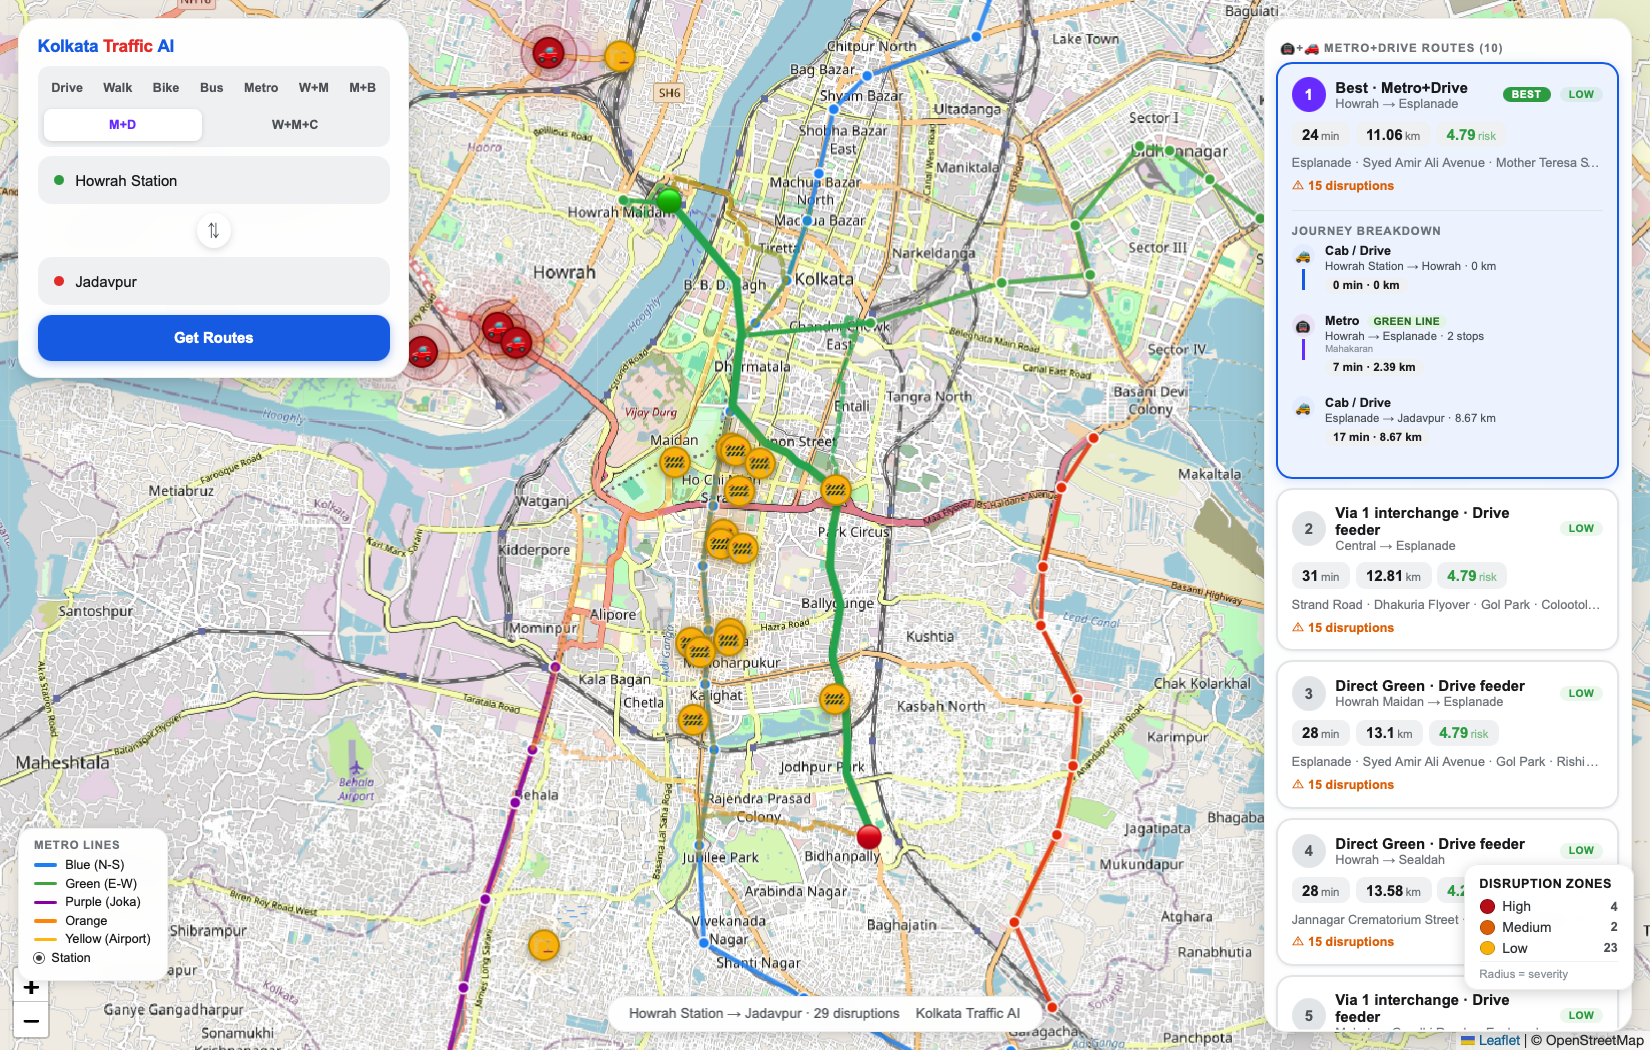
\includegraphics[width=1\linewidth]{ui2.png}
\caption{Step~2 --- routes coloured by risk; disruption panel populated.}
\label{fig:step2}
\end{figure}

% -------  Figure 4.3  -------
\begin{figure}[H]
\centering
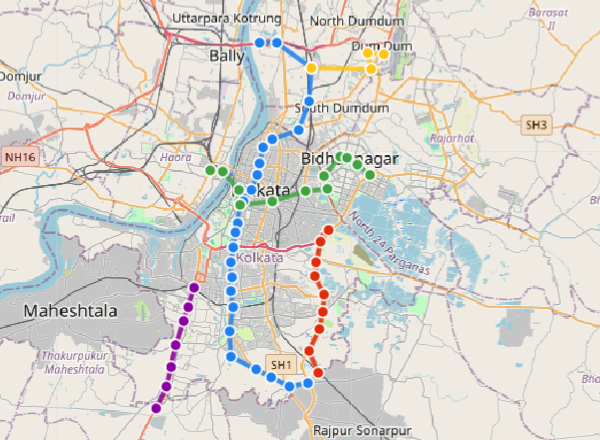
\includegraphics[width=1\linewidth]{ui_metro.png}
\caption{Metro overlay.}
\label{fig:metro}
\end{figure}

% -------  Figure 4.4  -------
\begin{figure}[H]
\centering
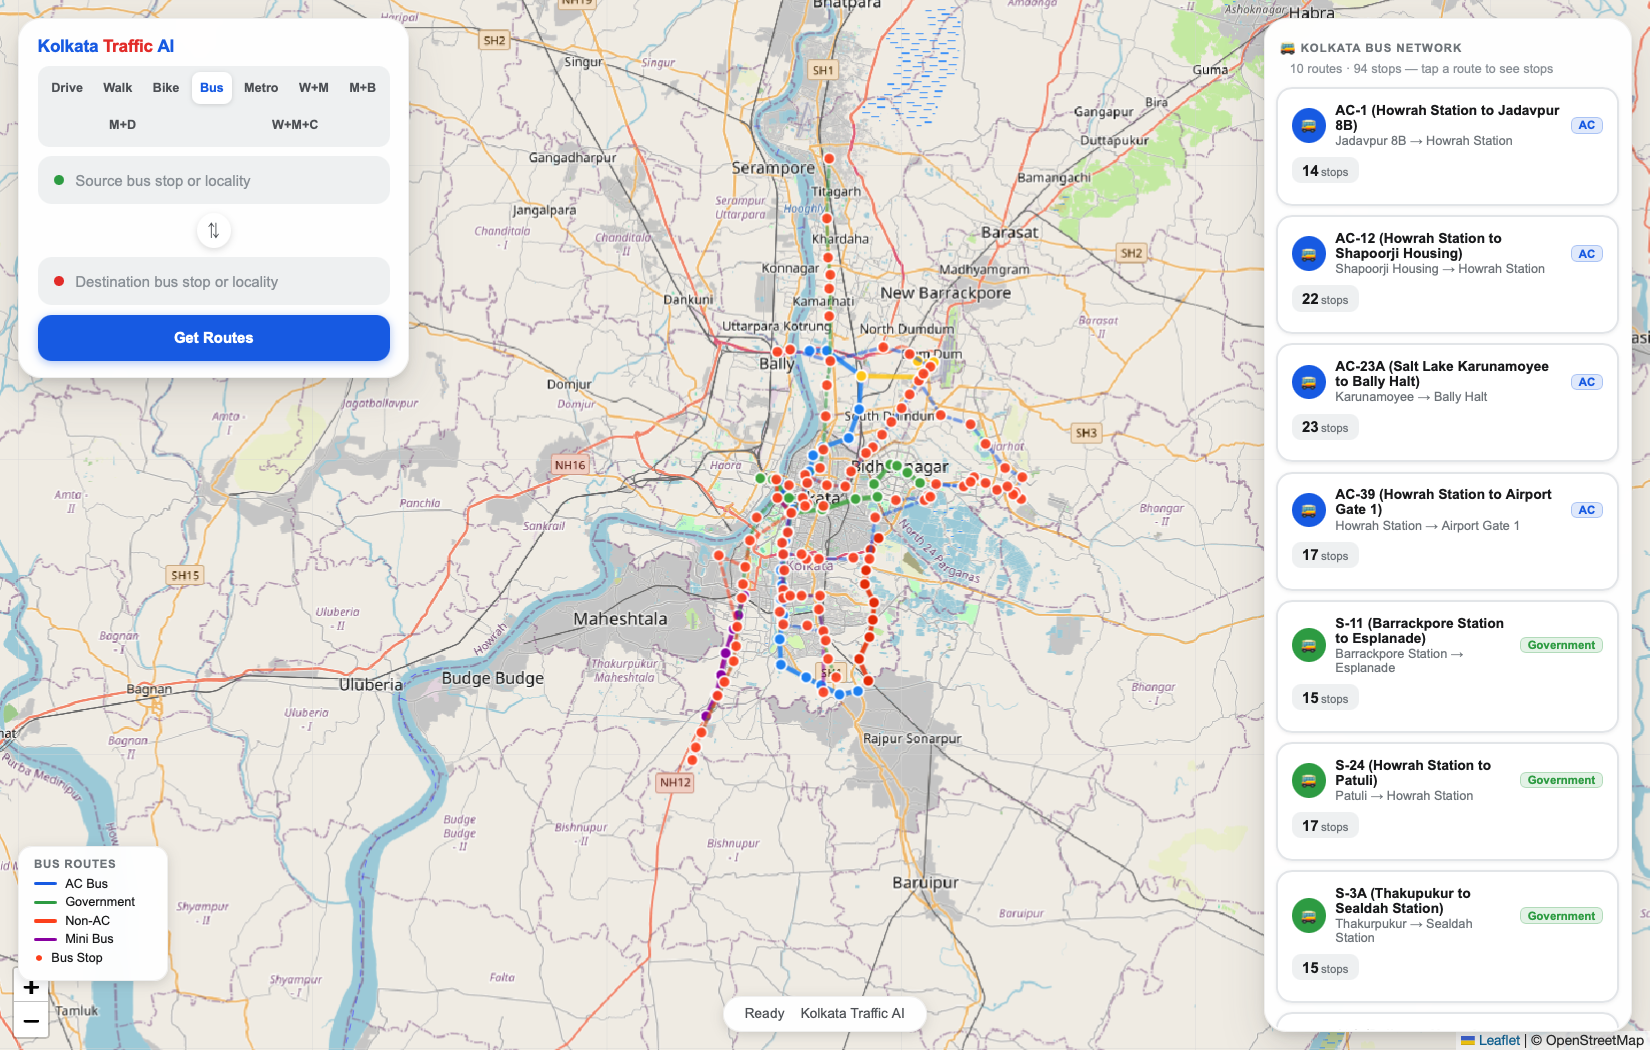
\includegraphics[width=1\linewidth]{bus.png}
\caption{Bus transit overlay and routing result.}
\label{fig:bus}
\end{figure}

% -------  Figure 4.5  -------
\begin{figure}[H]
\centering
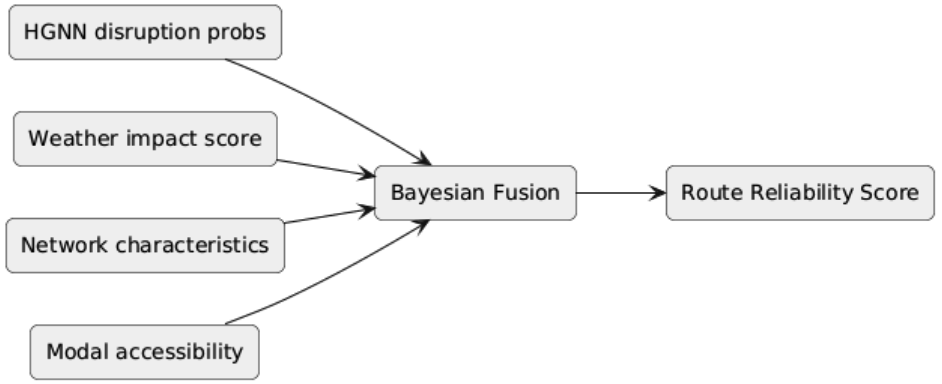
\includegraphics[width=\linewidth]{hgnn.png}
\caption{HGNN attention-based route explanation panel.}
\label{fig:explain}
\end{figure}

% -------------------------------------------------------------------
\section{Research Poster}
% -------------------------------------------------------------------

\noindent
The poster below was submitted as part of the GRISHMA programme deliverables.
It summarises the system architecture, methodology, and key findings.

\newpage
\thispagestyle{empty}
% Replace poster.pdf with your actual file when ready:
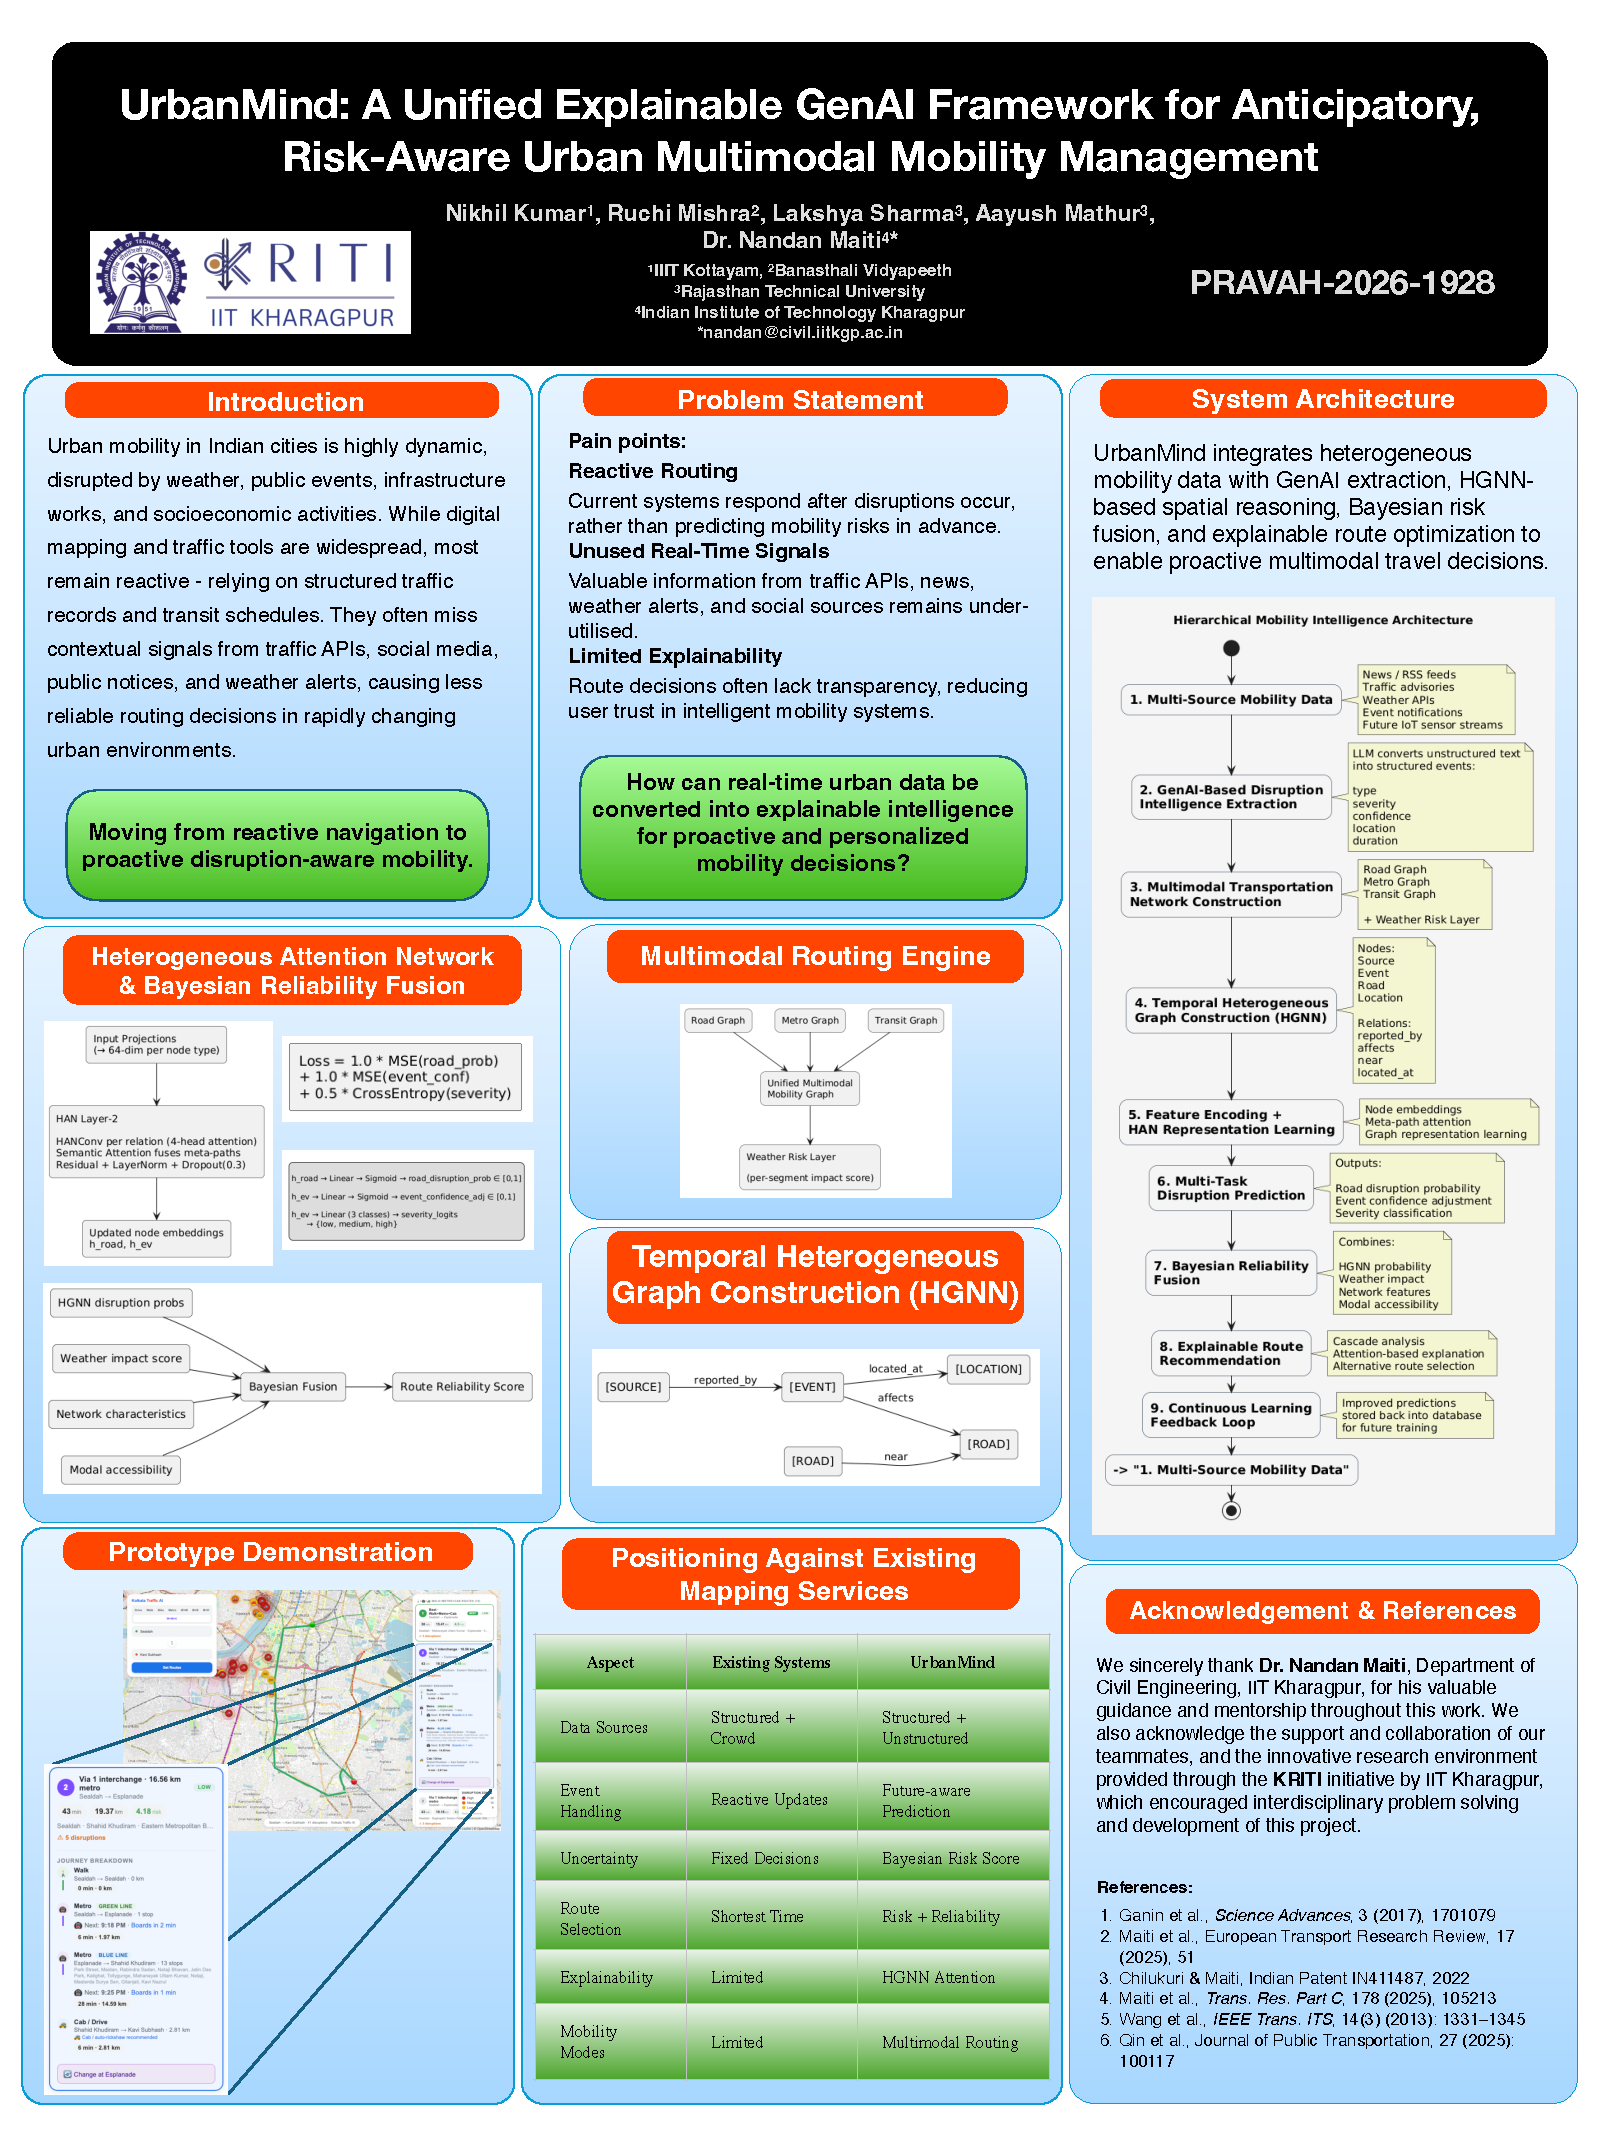
\includepdf[pages=1,scale=0.95]{Poster.pdf}
\newpage
